\documentclass[12pt, a4paper]{article}
\usepackage[outputdir=out]{minted}
\usepackage[utf8]{inputenc}
\usepackage{geometry}
\usepackage[italian]{babel}
\usepackage{graphicx}
\usepackage[belowskip=-15pt,aboveskip=0pt]{caption}

\graphicspath{{images/}}

\geometry {   
    top=20mm,
    bmargin=20mm
}
\begin{document}

\begin{titlepage}
    \centering

    \vspace{0.5cm} {
        \large Politecnico di Milano\\
    }

    \vspace{5cm} {
        \huge {
            Progetto di Reti Logiche 2021/2022\\
        }
        \vspace{0.5cm}
        \large {Scaglione Prof. Salice}
    }

    \vspace{2cm} {
        \large
        Edoardo Fullin ( Codice Persona 10677606)
    }

    \vspace*{\fill}
    \today

\end{titlepage}

\tableofcontents

\pagebreak

\section{Introduzione}

\subsection{Descrizione del progetto}

Lo scopo del progetto è il design, tramite linguaggio VHDL di un modulo hardware sintetizzabile per FPGA
in grado di applicare ad una sequenza di parole in input un codice convoluzionale $1/2$, che 
può essere implementato attraverso la macchina a stati finiti in figura.


\begin{figure}[!ht]
    \centering
    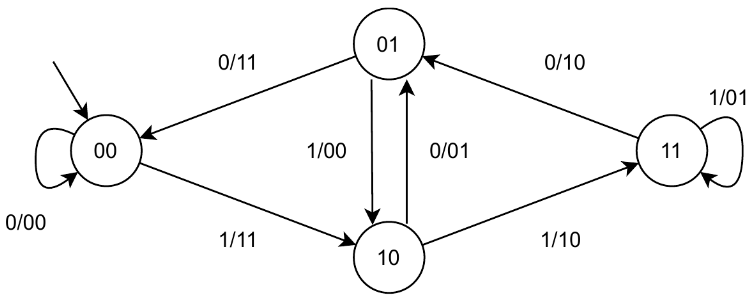
\includegraphics[scale=0.7]{convoluzionatore_1_2_fsm.png}
    \caption{FSM convoluzionatore $1/2$}
    \label{fig:fsm_conv}
\end{figure}

Il modulo deve quindi restituire in output (scrivendo in memoria) le uscite della macchina a stati finiti,
bit per bit. % dire meglio

\subsection{Esempio}

La FSM prende in input la parola \verb+11001011+, che deve essere serializzata come
1 al tempo 0, 1 al tempo 1, 0 al tempo 2 e così via.
La macchina quindi, partendo dallo stato di reset 00 andrà nello stato 10 alla lettura
del primo 1 producendo in output 11, passerà poi nello stato 3 producendo 10, nello stato 01
producendo 10 e nello stato 00 producendo 11.
Il primo byte di output sarà quindi 11100111, che dovrà essere scritto in memoria.
Si nota quindi facilmente che la lunghezza della sequenza di output è esattamente doppia di quella 
dell'input.

\pagebreak

\subsection{Specifiche del modulo da realizzare}

Il modulo da descrivere è sincrono sincronizzato su un clock 'globale', non include la memoria su cui viene effettuato input/output e
deve implementare la seguente interfaccia verso l'esterno:

\begin{minted}[]{vhdl}
    
    entity project_reti_logiche is
        port (
            i_clk : in std_logic;
            i_rst : in std_logic;
            i_start : in std_logic;
            i_data : in std_logic_vector(7 downto 0);
            o_address : out std_logic_vector(15 downto 0);
            o_done : out std_logic;
            o_en : out std_logic;
            o_we : out std_logic;
            o_data : out std_logic_vector (7 downto 0)
        );
    end project_reti_logiche;

\end{minted}

In particolare:

\begin{itemize}
    \item \texttt{i\_clk} è il segnale di clock, generato dall'esterno
    \item \texttt{i\_rst} è il segnale di reset
    \item \texttt{i\_start} è il segnale di inizio sequenza
    \item \texttt{i\_data} è il byte in arrivo dalla memoria RAM
    \item \texttt{o\_address} è l'indizzo di memoria da cui si vuole leggere/scrivere
    \item \texttt{o\_done} è il segnale di fine computazione
    \item \texttt{o\_en} è il segnale di enable per la memoria RAM
    \item \texttt{o\_we} è il segnale di scrittura per la memoria RAM
    \item \texttt{o\_data} è il byte da scrivere in memoria RAM
\end{itemize}

\pagebreak

\section{Architettura}

\subsection{Macchina a stati}

Il modulo è composto da una macchina a 14 stati il cui compito è quello di generare
i segnali di controllo in grado di attivare o disattivare le parti del datapath atte a
svolgere la funziona richiesta in quello specifico punto dell'esecuzione.\\

La macchina a stati è descritta come in figura, quando non è presente una label sulle transizioni
si intende che la transizione è incondizionata oppure, in presenza di altre transizioni
in uscita dallo stesso stato, quando la condizione associata all'altra transizione è falsa.
E' inoltre presente, ma non riportata nel diagramma, una transizione da tutti gli stati 
verso \texttt{SINIT} quando \texttt{i\_rst = 1}

\begin{figure}[!h]
    \centering
    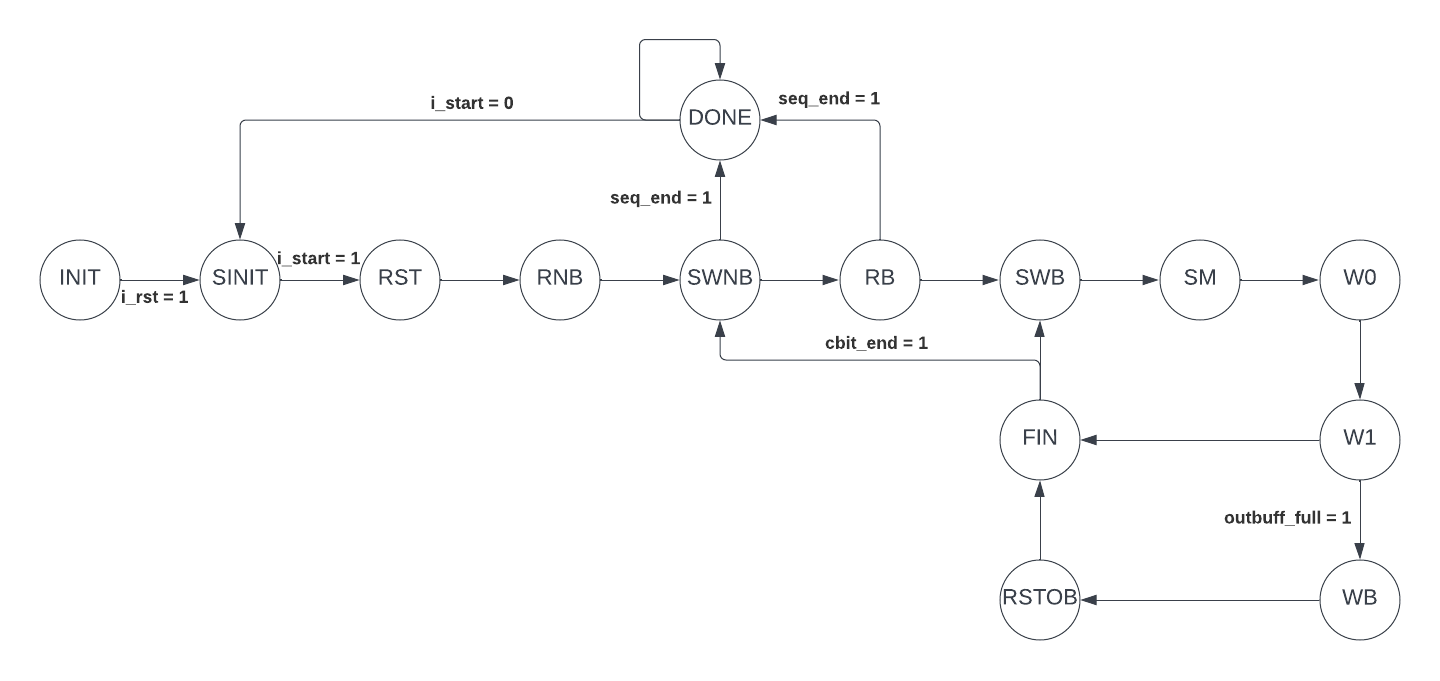
\includegraphics[scale=0.3]{fsm_controllo.png}
    \label{fig:ctrl_fsm}
    \caption{FSM di controllo}
    
\end{figure}

\subsubsection{INIT}
Stato iniziale in cui si trova la macchina prima dell'avvio dell'esecuzione.
I segnali di controllo sono tutti disattivati

\subsubsection{SINIT}
Stato in cui si trova la macchina prima dell'avvio di una nuova sequenza
I segnali di controllo sono tutti disattivati

\subsubsection{RST}
Reset di tutte le memoria interne al datapath per riportare rendere il datapath pronto per
una nuova sequenza. 
I segnali di controllo attivi sono:
\begin{itemize}
    \item \texttt{sm\_rst} che resetta stato corrente e uscita corrente del convoluzionatore
    \item \texttt{curr\_mux} ad 11 che resetta a la posizione corrente
    \item \texttt{outbuff\_rst} che resetta il buffer di output
    \item \texttt{outbuff\_load} che è necessario per resettare il bufferi di output
\end{itemize}

\subsubsection{RNB}
Lettura del numero di byte dalla RAM ad indirizzo 0.
I segnali di controllo attivi sono:
\begin{itemize}
    \item \texttt{nbytes\_load} che attiva il registro che salva il numero di byte
    \item \texttt{curr\_mux} ad 10 che fa avanzare la posizione corrente al prossimo byte
\end{itemize}

\subsubsection{SWNB}
Verifica lo stato corrente ed il termine della sequenza.
I segnali di controllo sono tutti disattivati

\subsubsection{RB}
Lettura del byte corrente e memorizzazione.
I segnali di controllo attivi sono:
\begin{itemize}
    \item \texttt{sr\_byte\_load} che attiva la lettura del registro che contiene il byte
\end{itemize}

\subsubsection{SWB}
Stato di stallo, in attesa che il byte veng letto con successo.
I segnali di controllo attivi sono:
\begin{itemize}
    \item \texttt{sr\_byte\_load} che attiva la lettura del registro che contiene il byte
\end{itemize}

\subsubsection{SM}
Il bit corrente è ora presente all'ingresso del convoluzionatore, che viene abilitato e viene
generato l'output relativo a quel bit.
I segnali di controllo attivi sono:
\begin{itemize}
    \item \texttt{sr\_ena} che attiva il registro serializzatore
    \item \texttt{sm\_ena} che attiva il convoluzionatore
\end{itemize}

\subsubsection{W0 e W1}
I bit di output vengono scritti nell'output buffer.
Al termine della scrittura si verifica il segnale \texttt{outbuff\_full} per decidere
se è necessario scrivere il bufferi di output in memoria.
I segnali di controllo sono:
\begin{itemize}
    \item \texttt{sm\_w\_sel} rispettivamente a 0 in W0 e 1 in W1 che indica se viene 
                              scritto il bit 0 alla posizione corrente o il bit 1 alla posizione corrente + 1
    \item \texttt{outbuff\_load} che abilita la scrittura nel bufferi di output
\end{itemize}

\subsubsection{WB}
Scrittura in memoria del buffer di output
I segnali di controllo attivi sono:
\begin{itemize}
    \item \texttt{writesel} che attiva il la scrittura in memoria e genera l'indirizzo corretto
\end{itemize}

\subsubsection{RSTOB}
Reset del buffer di output
I segnali di controllo attivi sono:
\begin{itemize}
    \item \texttt{outbuff\_rst} che resetta il buffer di output
    \item \texttt{outbuff\_load} che è necessario per resettare il bufferi di output
\end{itemize}

\subsubsection{FIN}
Il singolo bit è stato processato, viene avanzato il contatore.
Si verifica il segnale \texttt{cbit\_end} per decidere se è necessario passare alla lettura del
prossimo byte oppure del prossimo bit.
I segnali di controllo attivi sono:
\begin{itemize}
    \item \texttt{curr\_mux} a 01 che avanza il contatore di una posizione
\end{itemize}

\subsubsection{DONE}
La sequenza è terminata, in attesa di i\_start o i\_rst per iniziare una nuova sequenza.
I segnali di controllo attivi sono:
\begin{itemize}
    \item \texttt{o\_done} a 1 segnala il termine della computazione
\end{itemize}

\end{document}